\documentclass[runningheads]{llncs}

\usepackage[T1]{fontenc}
\usepackage{graphicx}
\usepackage{booktabs}
\usepackage{amsmath}
\usepackage{amssymb}
\usepackage{microtype}
\usepackage{xcolor}
\usepackage[font=small,skip=3pt]{caption}
\renewcommand{\arraystretch}{0.97}
\setlength{\textfloatsep}{9pt plus 2pt minus 2pt}
\setlength{\floatsep}{9pt plus 2pt minus 2pt}
\setlength{\intextsep}{9pt plus 2pt minus 2pt}
\setlength{\abovecaptionskip}{4pt}
\setlength{\belowcaptionskip}{2pt}
\renewcommand{\topfraction}{0.92}
\renewcommand{\bottomfraction}{0.75}
\renewcommand{\textfraction}{0.06}
\renewcommand{\floatpagefraction}{0.95}
\renewcommand{\dbltopfraction}{0.92}
\makeatletter
\renewcommand\subparagraph{\@startsection{subparagraph}{5}{\parindent}%
  {3.25ex \@plus 1ex \@minus .2ex}{-1em}{\normalfont\normalsize\bfseries}}
\makeatother
\usepackage{titlesec}
\titlespacing*{\section}{0pt}{7pt plus 1pt minus 1pt}{4pt}
\titlespacing*{\subsection}{0pt}{6pt plus 1pt minus 1pt}{3pt}
\titlespacing*{\paragraph}{0pt}{5pt plus 1pt minus 1pt}{1em}
\usepackage{url}
\usepackage[hidelinks]{hyperref}
\renewcommand\UrlFont{\color{blue}\rmfamily}

\begin{document}

\title{Reharvester: A Local-First System for Interactive\\ Research-Literature Discovery}

\titlerunning{Reharvester: Local-First Research-Literature Discovery}

\author{Yongyuth Chuankhuntod \and
Anirach Mingkhwan}

\authorrunning{Y. Chuankhuntod and A. Mingkhwan}

\institute{Faculty of Industrial and Technology Management,\\
King Mongkut's University of Technology North Bangkok (Prachinburi Campus), Prachinburi, Thailand\\
\email{\{yongyuth.c,anirach.m\}@kmutnb.ac.th}}

\maketitle

\begin{abstract}
Keeping pace with a fast-growing research literature is increasingly difficult, and
the cloud services that promise to help are opaque, non-portable, and require that
sensitive reading lists leave the user's machine. We present Reharvester, a
local-first system that turns a keyword or abstract query into an interactive map of a
research field with no analysis delegated to an external service. Reharvester harvests
bibliographic records, assembles them into a navigable knowledge graph, surfaces
emerging keyword trends against an explicit null model, and exposes the corpus
through a wiki-linked reader backed by retrieval-augmented generation over the graph.
Bibliographic harvesting is the only networked step; indexing, graph
construction, analysis, and question answering all execute on the user's hardware, and
the system is organised as a capability ladder that degrades rather than fails when
compute or models are unavailable. We evaluate a complete implementation on a 34{,}397-paper corpus spanning 2013--2026.
The whole pipeline builds in 25\,s on a 16-core laptop, and the capability ladder
retains 77\,\% of full known-item recall using nothing but an inverted index. Hybrid
retrieval with graph expansion reaches 0.958 recall@10 on known-item search and improves
nDCG@10 by 0.047 (95\,\% CI $[0.032, 0.061]$) over TF-IDF on a pooled-judgment topical
task. Two results temper the design: graph expansion yields no significant gain in
context quality over flat hybrid retrieval at equal token budget, and the exact
$k$-nearest-neighbour backbone scales as $n^{2.01}$, which we address with an
inverted-index pruning variant that scales as $n^{1.16}$ while retaining 82\,\% of exact
edges. The result is literature exploration that is reproducible, private, and
air-gappable.

\keywords{Literature discovery \and Knowledge graph \and Local-first software \and
Retrieval-augmented generation \and Research-gap analysis \and Keyword trends.}
\end{abstract}

\section{Introduction}
\label{sec:intro}

The volume of published research outpaces any individual's capacity to read it. A
researcher entering an unfamiliar subfield faces two problems: finding the handful of
papers that matter, and building a mental model of how the subfield is
organised---which communities exist, which are converging, which vocabulary has just
appeared. Contemporary discovery tools address the first well and the second only
incidentally.

They also centralise both the data and the reasoning. A query typed into a hosted
service leaves the user's machine, and so does the reading list it accumulates; for
work on unpublished results or sensitive data, that egress is a reason not to use the
tool at all. Centralisation also hides the ranking logic, so a result set cannot be
audited, reproduced, or cited as a method: when a service changes its model, last
year's literature review is no longer reproducible, and nothing in the artefact records
that it changed.

Local-first software \cite{kleppmann2019} offers the alternative stance: the user's
device holds the primary copy of the data and remains functional without a network. We
apply that stance to literature discovery. Reharvester reframes the task as a local,
inspectable pipeline: after an initial harvest, graph construction, trend analysis,
retrieval, and question answering all execute on the user's hardware. The design commitment we make,
and test, is that the system should never present a hard capability cliff: a user with
a 90\,MB neural encoder should get better results than a user without one, but the
user without one should still get a working system rather than an error.

We contribute (i) a local-first architecture organised as an explicit \emph{capability
ladder}, in which each tier adds a dependency and every tier below remains a complete
system; (ii) a trend-and-gap analytic layer pairing smoothed prevalence growth and burst
detection with a \emph{specificity} filter, scoring candidate gaps against a permutation
null rather than a raw density threshold; (iii) an evaluation on 34{,}397 papers covering
retrieval on two tasks with independent ground truth, context quality at fixed budget,
degradation, and scaling with measured exponents; and (iv) two negative results that
constrain the design---graph expansion does not improve retrieval-augmented context at
equal budget, and the exact backbone is quadratic, for which we give a near-linear
replacement.

\section{Related Work}
\label{sec:related}

\paragraph{Science mapping.}
VOSviewer \cite{eck2009} and CiteSpace \cite{chen2005} established the interactive
co-citation map as the standard artefact, These are desktop applications, local in the trivial sense,
but they consume curated citation databases and treat the map as the endpoint.
Reharvester treats it as an index into a reader: the graph is the substrate for
retrieval and question answering, not only for visual inspection. Open corpora make this
possible---S2ORC \cite{lo2020} and OpenAlex \cite{priem2022}---though our ingestion
stage is thin, and any source yielding titles, abstracts, authors, and dates can drive
the pipeline.

\paragraph{Retrieval.}
Sparse lexical retrieval remains a strong baseline, with BM25 \cite{robertson2009} the
reference method. Dense retrieval \cite{karpukhin2020a,izacard2021} now dominates;
scientific-domain \cite{beltagy2019a} and general sentence encoders \cite{reimers2019a}
supply the embeddings, benchmarks \cite{thakur2021} govern model selection, and
approximate nearest-neighbour indexes \cite{malkov2020} make dense search tractable.
Hybrid systems combine both signals, most simply through reciprocal rank fusion
\cite{cormack2009}. Our contribution is not a new retriever but a measurement of how
these components behave when the constraint is one consumer machine and every tier
must still work without the one above it.

\paragraph{Retrieval-augmented generation.}
RAG \cite{lewis2020} grounds generation in retrieved evidence, mitigating the long-tail
knowledge gaps of parametric models \cite{kandpal2022}; refinements address long-context
position sensitivity \cite{liu2024} among much else, open-weights models
\cite{jiang2023} make local generation feasible, and automated evaluation \cite{es2024}
informs our metric design. Most relevant is graph-structured RAG: GraphRAG
\cite{edge2024} builds an entity graph for query-focused summarisation and HippoRAG
\cite{gutirrez2024a} uses a graph as associative memory; both report that graph structure
helps. We test the same idea for a document-level semantic backbone under a fixed token
budget and---contrary to our expectation---find no significant benefit
(Section~\ref{sec:discussion}).

\paragraph{Trends, gaps, and reproducibility.}
Burst detection in document streams \cite{kleinberg2003} locates the moment a topic
emerges. Structural-hole theory \cite{burt2004} motivates reading sparse regions
between dense communities as opportunity, and community detection \cite{blondel2008}
provides the machinery. Our analytic layer adds two guards absent from the tools we
surveyed: a specificity filter and an explicit null model. Separately, both FAIR data practice and systematic-review
reporting standards require a search to be describable and repeatable, which a hosted
service whose model changes silently cannot satisfy.

\section{System Design}
\label{sec:design}

Reharvester is a five-stage pipeline (Fig.~\ref{fig:overview}a) in which each stage
writes a durable local artefact, so any stage can be re-run, inspected, or replaced
without re-running those before it.

\begin{figure}[htbp]
\centering
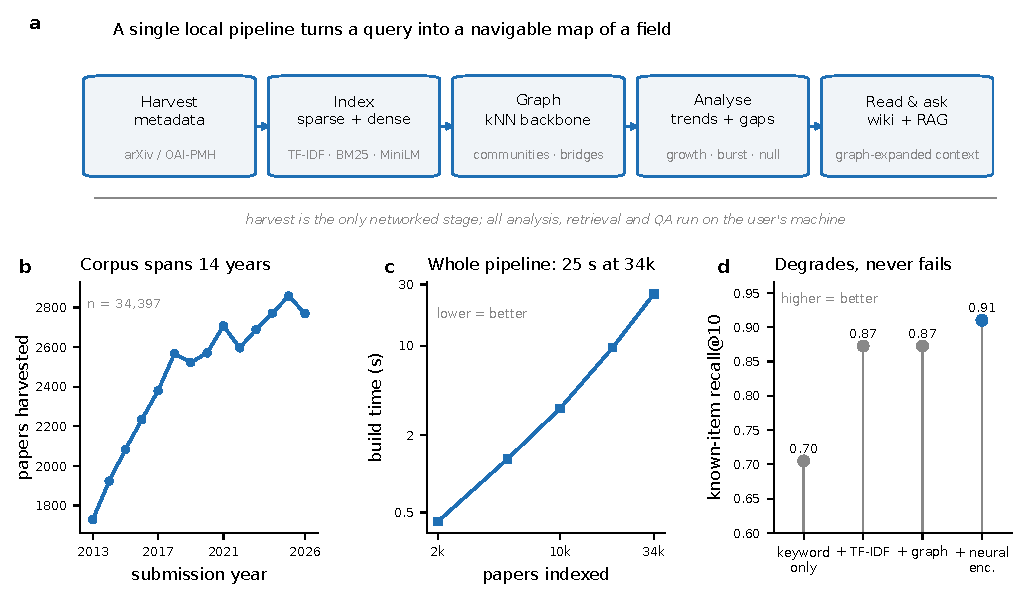
\includegraphics[width=0.92\textwidth]{fig1_overview.pdf}
\caption{System overview. (a) The five pipeline stages; harvesting is the only stage
that contacts the network, and everything downstream of it runs locally. (b) The evaluation corpus, harvested from five arXiv categories, spans
2013--2026 ($n = 34{,}397$ after deduplication and abstract-length filtering).
(c) End-to-end build time for indexing, graph construction, community detection and
trend analysis on a 16-core Apple-silicon laptop. (d) Known-item recall@10 across the
capability ladder ($n = 400$ queries): each tier adds one dependency, and the tier
with no model and no graph still answers 70.5\,\% of queries.}
\label{fig:overview}
\end{figure}

\paragraph{Harvest and index.}
Ingestion pulls title, abstract, authors, categories, and date from an open API into a
flat local store, deduplicating on the version-stripped identifier; this is the only
stage that touches the network, and afterwards the system is fully functional offline. It
retrieved 37{,}006 records in 928\,s, a rate set by the source API's politeness delay
rather than local compute. Three indexes are then built over abstracts: a TF-IDF index
(unigrams and bigrams, sublinear term-frequency scaling) that supports cosine ranking and
supplies the vector space for the graph; a BM25 index \cite{robertson2009} with different
failure modes; and a dense index encoding each abstract into 384 dimensions with a compact
sentence encoder \cite{reimers2019a}. These cost 5.0\,s, 1.6\,s, and 388\,s respectively;
the dense index is by far the most expensive stage, which is why the ladder treats it as
optional.

\paragraph{Graph.}
The semantic backbone is a mutual $k$-nearest-neighbour graph over the TF-IDF space
with $k = 8$, edges weighted by cosine similarity, yielding 203{,}100 edges. A
co-authorship layer adds 269{,}295 edges over 71{,}988 distinct author strings, with
authors on more than 60 papers excluded to limit name-collision effects. Louvain
community detection \cite{blondel2008} partitions the backbone into 35 communities,
each labelled by its centroid's highest-weight terms, and a per-node bridge
score---the fraction of a node's edge weight crossing a community boundary---identifies
papers between topics, operationalising the structural-hole intuition \cite{burt2004}
at document level. The backbone, not the raw index, makes the system navigable: it
converts a ranked list into a neighbourhood the user can walk.

\paragraph{Analyse.}
\label{sec:analytics}
This layer answers two questions a ranked list cannot: what vocabulary is emerging,
and where are the gaps? Both required care, and both went through a failed first
version we report because the failure is instructive.

A naive $n$-gram extractor that removes stopwords and then forms bigrams from the
surviving token stream generates phrases that never occurred in the text: in our first
run ``models llms'' was the fastest-rising bigram in the corpus with 1{,}579 late-window
occurrences, an artefact of joining ``\dots models.'' to ``LLMs have\dots'' across a
sentence boundary. Our extractor therefore splits on sentence and clause punctuation
first, forms $n$-grams only within maximal runs of non-stopword tokens, and discards
residual \LaTeX{} control words, which otherwise appear as burst terms
(\texttt{textbf} peaked in 2026 with burst weight 16.4).

Prevalence growth compares a term's document-frequency share between an early and a late
window. An unsmoothed log-ratio is infinite for any term absent from the early
window---exactly the interesting case---so we smooth with $\alpha = 0.5$ pseudo-documents,
taking $\mathrm{lift}(t) = [(n_{\text{late}}(t)+\alpha)/D_{\text{late}}] \,/\,
[(n_{\text{early}}(t)+\alpha)/D_{\text{early}}]$ where $n_w(t)$ counts documents in
window $w$ containing $t$ and $D_w$ counts documents in that window. Raw counts are
reported alongside so a reader can distinguish a new phrase from a merely growing one.

Burst and growth statistics are otherwise dominated by discourse vocabulary
(``underexplored'', ``findings highlight'') that rises because writing conventions
change, not because a topic emerged. We filter on the normalised entropy of a term's
distribution over communities,
$S(t) = -\sum_{c} p(c \mid t) \log p(c \mid t) \,/\, \log |C|$, retaining terms with
$S \le 0.80$: a term spread evenly over all communities has $S \approx 1$, a topical
term concentrates. The median unigram specificity here is 0.778, so this is a mild
filter that nonetheless removes the worst offenders.

Finally, a research gap is a pair of communities whose documents read alike but between
which few links exist. Scoring this as raw cross-edge density conflates a real gap with
the fact that small communities have few edges: our first version ranked a small
recipe-and-food community against nearly everything else. We instead compare the observed
cross-community edge count against a null obtained by permuting community labels over the
fixed graph 200 times---preserving the degree sequence and the community sizes---and
report a $z$-score, taking as candidates the pairs with high centroid cosine similarity
and $z < -2$.

\paragraph{Read and ask.}
The reader presents papers with wiki-style links along backbone edges, so navigation
follows semantic adjacency rather than a ranked list. Question answering assembles a
context set under a fixed token budget---seeding with hybrid retrieval, expanding along
the backbone---and hands it to a local open-weights model \cite{jiang2023}. We evaluate
the context assembly rather than the generated prose, since context quality is the part
our design choices control.

\subsection{The capability ladder}
\label{sec:ladder}
A local-first system runs on hardware it does not choose. Reharvester is therefore built
as four tiers, each a complete system: \textbf{T0}, an inverted index only, with boolean
candidate generation and token-overlap ranking, needing nothing beyond the standard
library; \textbf{T1}, adding a TF-IDF vectoriser; \textbf{T2}, adding the $k$-NN
backbone, which enables neighbourhood expansion and the community and trend analytics;
and \textbf{T3}, adding a neural sentence encoder ($\approx$\,90\,MB). The ladder is not
a fallback path taken on error but a configuration the user chooses.

\section{Implementation and Evaluation}
\label{sec:impl}

The implementation is Python~3.13 with NumPy, SciPy, scikit-learn, NetworkX, and
\texttt{rank\_bm25}; the optional dense tier uses \texttt{sentence-transformers} with a
384-dimensional MiniLM encoder. No component requires a GPU, and none issues a network
request after harvesting. All measurements were taken single-process on a 16-core
Apple-silicon laptop (macOS~26.5, 137\,GB RAM). Two choices deserve note: retrieval
indexes are built over \emph{abstracts only}, which makes the known-item task below a
genuine test at some cost in absolute accuracy; and the graph is built from the TF-IDF
space rather than the dense space, so the backbone, the communities, and every analytic
result depending on them remain available at tier~T2 with no neural model present.

\paragraph{Corpus.}
We harvested five arXiv categories---cs.IR, cs.DL, cs.CL, cs.SI, cs.DB---across
2013--2026, retaining records with abstracts longer than 200 characters; after
deduplication this gives 34{,}397 papers (Fig.~\ref{fig:overview}b), 1{,}729--2{,}858 per
year. The corpus is deliberately heterogeneous, spanning lexical retrieval, network
science, and database systems, so community structure is present but not trivially
separable.

\paragraph{Ground truth.}
Evaluating a discovery system without relevance assessors requires ground truth the
system under test did not produce; we use three sources, none derived from the machinery
being measured. In \textbf{Task A} (known-item retrieval) the query is a paper's title
and the single relevant document is its own abstract; because titles are excluded from
every index, this measures whether a retriever can bridge a short, differently-worded
query to the right document. In \textbf{Task B} (topical retrieval) the query is a
paper's abstract and relevance follows arXiv's own multi-label category assignment,
applied by authors and moderators independently of our system: grade 3 for the same
primary category and $\ge 2$ shared labels, 2 for the same primary category, 1 for
$\ge 2$ shared secondary labels, 0 otherwise. Sharing a single broad label is not
relevant, which keeps the task discriminative, and judgments are \emph{pooled}---the
ideal nDCG ranking comes from the union of all five systems' top-50 results, so no
system is scored against a reference derived from its own output. In \textbf{Task C}
(context quality) a gold set of five documents per seed is defined by proximity in a
\emph{character-4-gram} TF-IDF space---used by no retriever and not involved in building
the graph---further constrained to grade $\ge 2$ under the Task~B criterion. This metric
is the one most at risk of circularity, and the independent judge space is what removes
it: our first version defined gold sets from graph neighbourhoods and consequently
reported that graph expansion won. Confidence intervals are paired bootstrap with
5{,}000 resamples.

\section{Results}
\label{sec:results}

\subsection{Retrieval quality}
\label{sec:res:retrieval}

\begin{table}[htbp]
\centering\small
\caption{Retrieval quality. Task~A is known-item search over 500 queries; Task~B is
topical search over 400 queries with pooled graded judgments. P@10$_{\ge 2}$ counts only
high-relevance hits (grade $\ge 2$ of 3). Latency (ms/q) is mean wall-clock time per
query, single-threaded, including all constituent retrievals for hybrid methods. Best
value per column in bold.}
\label{tab:retrieval}
\setlength{\tabcolsep}{3.0pt}
\begin{tabular}{lcccccccc}
\toprule
& \multicolumn{3}{c}{Task A: known-item} & \multicolumn{4}{c}{Task B: topical} & \\
\cmidrule(lr){2-4}\cmidrule(lr){5-8}
Method & P@1 & R@10 & MRR & nDCG@10 & P@10 & P@10$_{\ge 2}$ & R@20 & ms/q \\
\midrule
TF-IDF            & 0.612 & 0.866 & 0.701 & 0.443 & 0.599 & 0.484 & 0.581 & 5.3 \\
BM25              & 0.758 & 0.918 & 0.817 & 0.435 & 0.588 & 0.475 & 0.568 & 32.2 \\
Dense (MiniLM)    & 0.700 & 0.924 & 0.779 & 0.485 & \textbf{0.669} & 0.532 & \textbf{0.659} & \textbf{2.1} \\
Hybrid (RRF)      & 0.760 & 0.950 & 0.837 & 0.476 & 0.642 & 0.521 & 0.610 & 39.7 \\
Hybrid + graph    & \textbf{0.762} & \textbf{0.958} & \textbf{0.839} & \textbf{0.490} & 0.666 & \textbf{0.536} & 0.645 & 39.7 \\
\bottomrule
\end{tabular}
\end{table}

On known-item search (Table~\ref{tab:retrieval}, Fig.~\ref{fig:retrieval}a) hybrid
retrieval with graph expansion reaches 0.958 recall@10, ahead of rank fusion alone
(0.950), dense retrieval (0.924), and BM25 (0.918); the ordering is unsurprising and the
graph contribution small. Topical search is more informative. Hybrid-plus-graph attains the best nDCG@10
(0.490), a paired-bootstrap difference against the TF-IDF baseline of $+0.047$ with
95\,\% CI $[0.032, 0.061]$. Dense retrieval alone attains 0.485 ($+0.041$, CI
$[0.023, 0.060]$)---statistically indistinguishable from the full hybrid
pipeline---at 2.1\,ms per query against 410.0\,ms, a factor of about 200. BM25 is the
only method that does not significantly beat TF-IDF here ($-0.009$, CI
$[-0.022, +0.005]$) despite being clearly better on known-item search: a lexical
ranker tuned for short queries does not transfer to a task whose query is a 200-word
abstract. The practical reading is that on any machine able to run the neural encoder,
dense retrieval alone is the right default, and the hybrid pipeline earns its
200-fold latency cost only where the last two points of nDCG matter.

\begin{figure}[htbp]
\centering
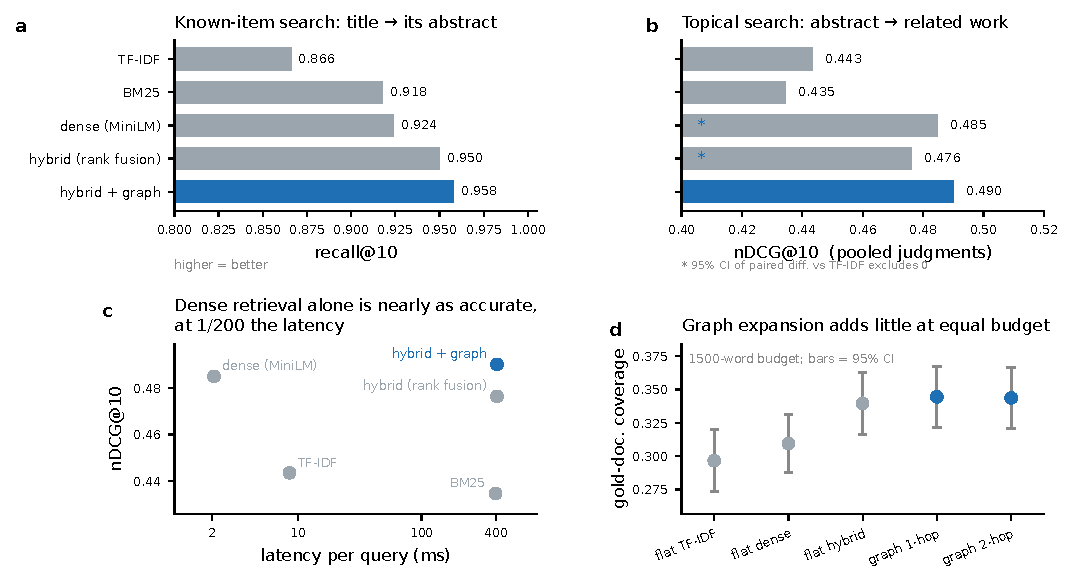
\includegraphics[width=0.86\textwidth]{fig3_retrieval.pdf}
\caption{Retrieval and context results. (a) Known-item recall@10, 500 queries.
(b) Topical nDCG@10, pooled graded judgments, 400 queries; asterisks mark methods whose
paired-bootstrap 95\,\% CI against TF-IDF excludes zero. (c) The quality--latency
trade-off. (d) Gold-document coverage under a 1{,}500-word budget, 250 seeds, 95\,\% CIs.}
\label{fig:retrieval}
\end{figure}

\subsection{Context quality: a negative result}
\label{sec:res:context}

Task~C tests the assumption behind graph-expanded RAG. Under a 1{,}500-word budget, flat
hybrid retrieval captures 0.340 of the gold set, one-hop graph expansion 0.344, and
two-hop 0.344; the paired-bootstrap difference for one-hop expansion over flat hybrid is
$+0.005$, CI $[-0.006, +0.015]$, no significant effect. Both flat single-retriever
baselines are significantly \emph{worse} than flat hybrid (TF-IDF $-0.043$, CI
$[-0.061, -0.025]$; dense $-0.030$, CI $[-0.049, -0.012]$), so the experiment has enough
power to detect differences of the size we hoped to see from the graph. A secondary
measurement shows the mechanism: averaged over seeds, flat TF-IDF context spans 4.00
distinct communities, flat hybrid 3.07, and one-hop expansion 2.73. Expansion along a
semantic backbone retrieves documents similar to those already retrieved, so at fixed
budget it trades topical diversity for local density---a trade that is approximately
neutral when the gold set is defined independently of the graph.

\subsection{The capability ladder}
\label{sec:res:ladder}

\begin{table}[htbp]
\centering\small
\caption{(a) Capability ladder on known-item retrieval, 400 queries; each tier adds one
dependency to the one above it. (b) End-to-end scaling, single process, with peak RSS
measured in an isolated subprocess per corpus size and exponents from a log--log fit
across the five sizes.}
\label{tab:ladder}
\begin{minipage}[t]{0.415\textwidth}
\centering
(a)\\[2pt]
\begin{tabular}{llcc}
\toprule
Tier & Adds & R@10 & P@1 \\
\midrule
T0 & inverted index   & 0.705 & 0.600 \\
T1 & + TF-IDF         & 0.873 & 0.635 \\
T2 & + $k$-NN graph   & 0.873 & 0.635 \\
T3 & + encoder        & 0.910 & 0.738 \\
\bottomrule
\end{tabular}
\end{minipage}\hfill
\begin{minipage}[t]{0.575\textwidth}
\centering
(b)\\[2pt]
\setlength{\tabcolsep}{3.4pt}
\begin{tabular}{lrrrrr}
\toprule
Papers & Index & $k$-NN & Louv. & Total & RSS \\
       & (s) & (s) & (s) & (s) & (MB) \\
\midrule
2{,}000  & 0.22 & 0.05  & 0.08 & 0.42  & 591 \\
5{,}000  & 0.58 & 0.32  & 0.22 & 1.30  & 1{,}075 \\
10{,}000 & 1.24 & 1.13  & 0.49 & 3.24  & 2{,}562 \\
20{,}000 & 2.73 & 4.85  & 1.31 & 9.65  & 3{,}401 \\
34{,}397 & 5.61 & 15.79 & 2.54 & 25.34 & 3{,}626 \\
\midrule
Exp. & $n^{1.13}$ & $n^{2.00}$ & $n^{1.21}$ & $n^{1.43}$ & $n^{0.69}$ \\
\bottomrule
\end{tabular}
\end{minipage}
\end{table}

The tier with no vector space, no graph, and no model answers 70.5\,\% of known-item
queries within the top ten---77\,\% of what the full neural tier achieves
(Table~\ref{tab:ladder}a). Adding the TF-IDF vectoriser recovers most of the remaining
gap (0.873), and the neural encoder adds a further 0.037 recall and a substantial
0.103 in P@1. Notably T3 is also the \emph{fastest} tier at query time (2.1\,ms),
because a 384-dimensional dense scan is cheaper than a sparse cosine over a
120{,}000-term vocabulary; its cost is paid once, at index time, as the 388\,s
encoding pass. Tier T2 does not change known-item accuracy at all, which is the honest reading: the backbone exists to support navigation, communities, and the
trend analytics, and should not be justified by retrieval numbers.

\subsection{Trends and gaps}
\label{sec:res:trends}

The fastest-rising bigrams over 2022--26 relative to 2013--17
(Fig.~\ref{fig:analytics}a) are ``graph neural'' (smoothed log$_2$ lift 9.26, 404
late-window documents), ``large language'' (9.00, 2{,}374), ``retrieval-augmented
generation'' (8.91, 317), and ``contrastive learning'' (8.36, 216); the steepest declines
are ``distributed representations'' ($-4.74$, 50 documents to 2), ``statistical machine''
($-4.37$, 70 to 4), and ``thomson reuters'' ($-6.38$, 31 to 0)---the last a vendor name
whose disappearance tracks a database rebranding rather than a scientific shift, a
reminder that the method detects vocabulary, not ideas. Trajectories make the
substitution legible: ``statistical machine'' peaks in 2015 at 0.96\,\% of abstracts and
reaches 0\,\% by 2024, while ``graph neural'' peaks at 3.87\,\% in 2023--24 and
``retrieval-augmented generation'' rises from zero to 5.05\,\% in 2025. The specificity
filter makes this readable: without it the top burst terms are ``prompt'' (legitimate)
followed by ``decouples'', ``aligns'', and ``underexplored''.

\begin{figure}[htbp]
\centering
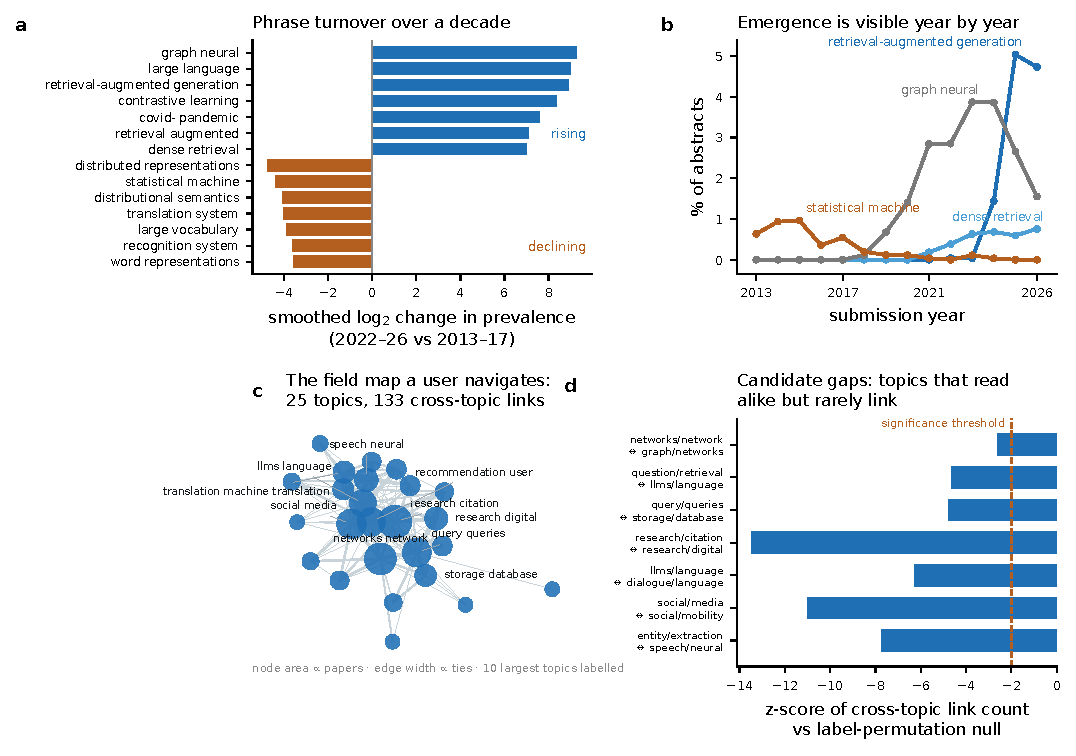
\includegraphics[width=0.83\textwidth]{fig2_analytics.pdf}
\caption{The analytic layer. (a) Seven fastest-rising and seven steepest-declining
bigrams by smoothed log$_2$ prevalence change (2022--26 vs 2013--17), after specificity
filtering. (b) Year-by-year prevalence of four phrases, showing substitution rather than
monotone growth. (c) The coarse-grained field map: 25 communities of $\ge$\,400 papers,
edges for inter-community links above threshold, ten largest topics labelled. (d) The
seven highest-similarity pairs whose cross-link count falls below a label-permutation
null; because 536 of 561 pairs cross $z < -2$, similarity rather than significance drives
this ranking.}
\label{fig:analytics}
\end{figure}

Fig.~\ref{fig:analytics}c--d show the coarse-grained map---25 communities of at least 400
papers, 133 inter-community links above threshold---and the top gap candidates. The
highest-similarity under-connected pairs are the two network-science communities (centroid
cosine 0.736; 927 cross-links against a null mean of 1{,}015, $z = -2.6$), question
answering against large language models (0.696; 697 vs.\ 833, $z = -4.7$), query
processing against storage systems (0.688; 892 vs.\ 1{,}064, $z = -4.8$), and citation
analysis against digital-library infrastructure (0.672; 1{,}045 vs.\ 1{,}616,
$z = -13.5$). Each names two communities that share vocabulary and methods but publish in
different venues. One limitation must be explicit: of 561 pairs, 536 reach $z < -2$,
because permuting labels destroys all topical structure and so makes nearly every real
pair look under-connected. The $z$-score is thus a weak filter and the ranking is carried
almost entirely by centroid similarity; a stronger null would preserve topical
assortativity, and we regard this result as a shortlist generator rather than a
hypothesis test.

\subsection{Scalability}
\label{sec:res:scaling}


The whole pipeline builds in 25.3\,s at 34{,}397 papers within 3.6\,GB of resident memory
(Table~\ref{tab:ladder}b), with indexing, community detection, and trend analysis all
near-linear ($n^{1.13}$, $n^{1.21}$, $n^{1.05}$). The exact $k$-NN backbone is not: it
scales as $n^{2.00}$, consistent with its brute-force all-pairs formulation, and dominates
total cost beyond about 10{,}000 papers---extrapolating the fit, a 500{,}000-paper corpus
would need roughly 53\,min for the backbone alone.

We therefore implemented an approximate backbone that prunes candidates using the
TF-IDF inverted index: for each document only its 24 highest-weight terms are probed,
rarest postings first, and the candidate pool is capped at 400 before exact cosine
scoring. This needs no external ANN library, preserving the local-first property. The
variant scales as $n^{1.16}$ against $n^{2.01}$ for the exact computation, crossing
over at roughly 20{,}000 papers and reaching a 1.97$\times$ speedup at 34{,}397
(8.25\,s vs.\ 16.24\,s). The fidelity cost is real and grows with corpus size: edge
recall against the exact graph falls from 0.941 at 5{,}000 papers to 0.815 at
34{,}397, and the adjusted mutual information between the resulting community
partitions falls from 0.749 to 0.624. The approximation is therefore appropriate for navigation and retrieval seeding, and
questionable for community-level analytics, where we default to the exact backbone.

\begin{figure}[htbp]
\centering
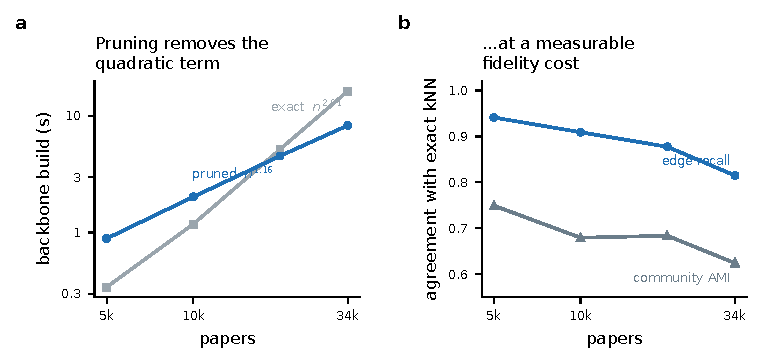
\includegraphics[width=0.72\textwidth]{fig4_scaling.pdf}
\caption{The backbone bottleneck. (a) Inverted-index candidate pruning reduces the
scaling exponent from $n^{2.01}$ to $n^{1.16}$, crossing over near 20k papers. (b) The
cost: edge recall and community agreement (AMI) against the exact backbone both degrade
as the corpus grows. Per-stage wall times are in Table~\ref{tab:ladder}b.}
\label{fig:scaling}
\end{figure}

\section{Discussion}
\label{sec:discussion}

Three claims survive our own attempts to break them. A full literature-mapping pipeline
over tens of thousands of papers is a 25-second local computation, not a service. The
capability ladder is real: the bottom rung retains 77\,\% of top-tier known-item recall
with no model and no graph, so a user on constrained hardware or inside an air gap gets
a working system. And on any machine that can run a 90\,MB encoder, dense retrieval
alone is the right default, within 0.005 nDCG of the full hybrid pipeline at 1/200 of
the latency.

Our negative result on context quality differs from reports that graph structure improves
RAG \cite{edge2024,gutirrez2024a}, and the difference is instructive rather than
contradictory. Those systems build graphs over \emph{entities} and use them to assemble
evidence that is topically distant but relationally connected; our backbone connects
\emph{whole documents} by lexical similarity, so expanding along it moves toward documents
resembling those already retrieved, which at fixed budget reduces topical diversity (3.07
to 2.73 communities per context) without improving coverage. The lesson is not that
graph-structured RAG fails but that the graph must encode a relation the retriever does
not already capture: a citation or entity layer satisfies that condition, a semantic
$k$-NN layer over the retriever's own features does not.

\paragraph{Limitations.}
Ground truth comes from arXiv category labels and an independent lexical space, not human
assessors; both are proxies, and category grading in particular rewards retrieving papers
from the same subfield rather than useful ones. Our corpus is five computer-science
categories from one repository, so community structure may be more separable than in an
interdisciplinary corpus, and the gap null model is weak as Section~\ref{sec:res:trends}
states. We evaluate context assembly rather than generated answers, so no claim is made
about end-to-end answer quality; doing so would need human judgment or an LLM-based
protocol \cite{es2024} whose own validity would need establishing. All timings come from
one machine class.

\paragraph{Future work.}
The most valuable addition is a citation layer, which our own negative result predicts
would make graph expansion effective; beyond that, a stronger null preserving topical
assortativity, incremental index and graph updates so a weekly harvest does not force a
rebuild, and a human study, since every claim here about what helps a researcher navigate
a field is currently an inference from automatic metrics.

\section{Conclusion}
\label{sec:conclusion}

Reharvester shows that interactive research-literature discovery does not require a
cloud service. A five-stage pipeline over 34{,}397 papers builds in 25\,s on a laptop,
produces a navigable field map with 35 communities and an auditable trend analysis, and
answers known-item queries at 0.958 recall@10. Organising the system as a capability
ladder rather than a monolith means it degrades instead of failing: 70.5\,\% recall@10
survives with nothing but an inverted index. Two measured negatives shape the design as
much as the positives---graph expansion over a document-similarity backbone does not
improve retrieval-augmented context at equal budget, and the exact backbone is
quadratic, needing the near-linear pruning variant we give. Because everything after
harvesting runs locally and every artefact is inspectable, a literature search performed
with Reharvester is something a researcher can hold, repeat, and cite.

\begin{credits}
\subsubsection{\ackname}
We thank the arXiv API maintainers, whose open interface makes local-first bibliographic
work possible. The authors declare no competing interests.
\end{credits}

\begingroup
\small
\setlength{\itemsep}{0pt}
\providecommand{\doi}[1]{}\renewcommand{\doi}[1]{}
\bibliographystyle{splncs04}
\bibliography{refs}
\endgroup

\end{document}
